\subsection{Parameters identification results}
\label{subsec:parameters_identification_results}

Once the previously explained procedure has been applied to all the natural frequencies of the system (consider for each one, every experimental FRFs at our disposal), we can reassemble the identified parameters so to compute the numerical FRFs of the system.

In the following figures, the result obtained considering the FRF relative to an input in $x_k = 1.0m$ and an output in $y_j = 0.6m$ is shown.

\begin{center}
    \huge{Plot to be replaced with the correct one.}
\end{center}

\begin{figure}[H]
    \centering
    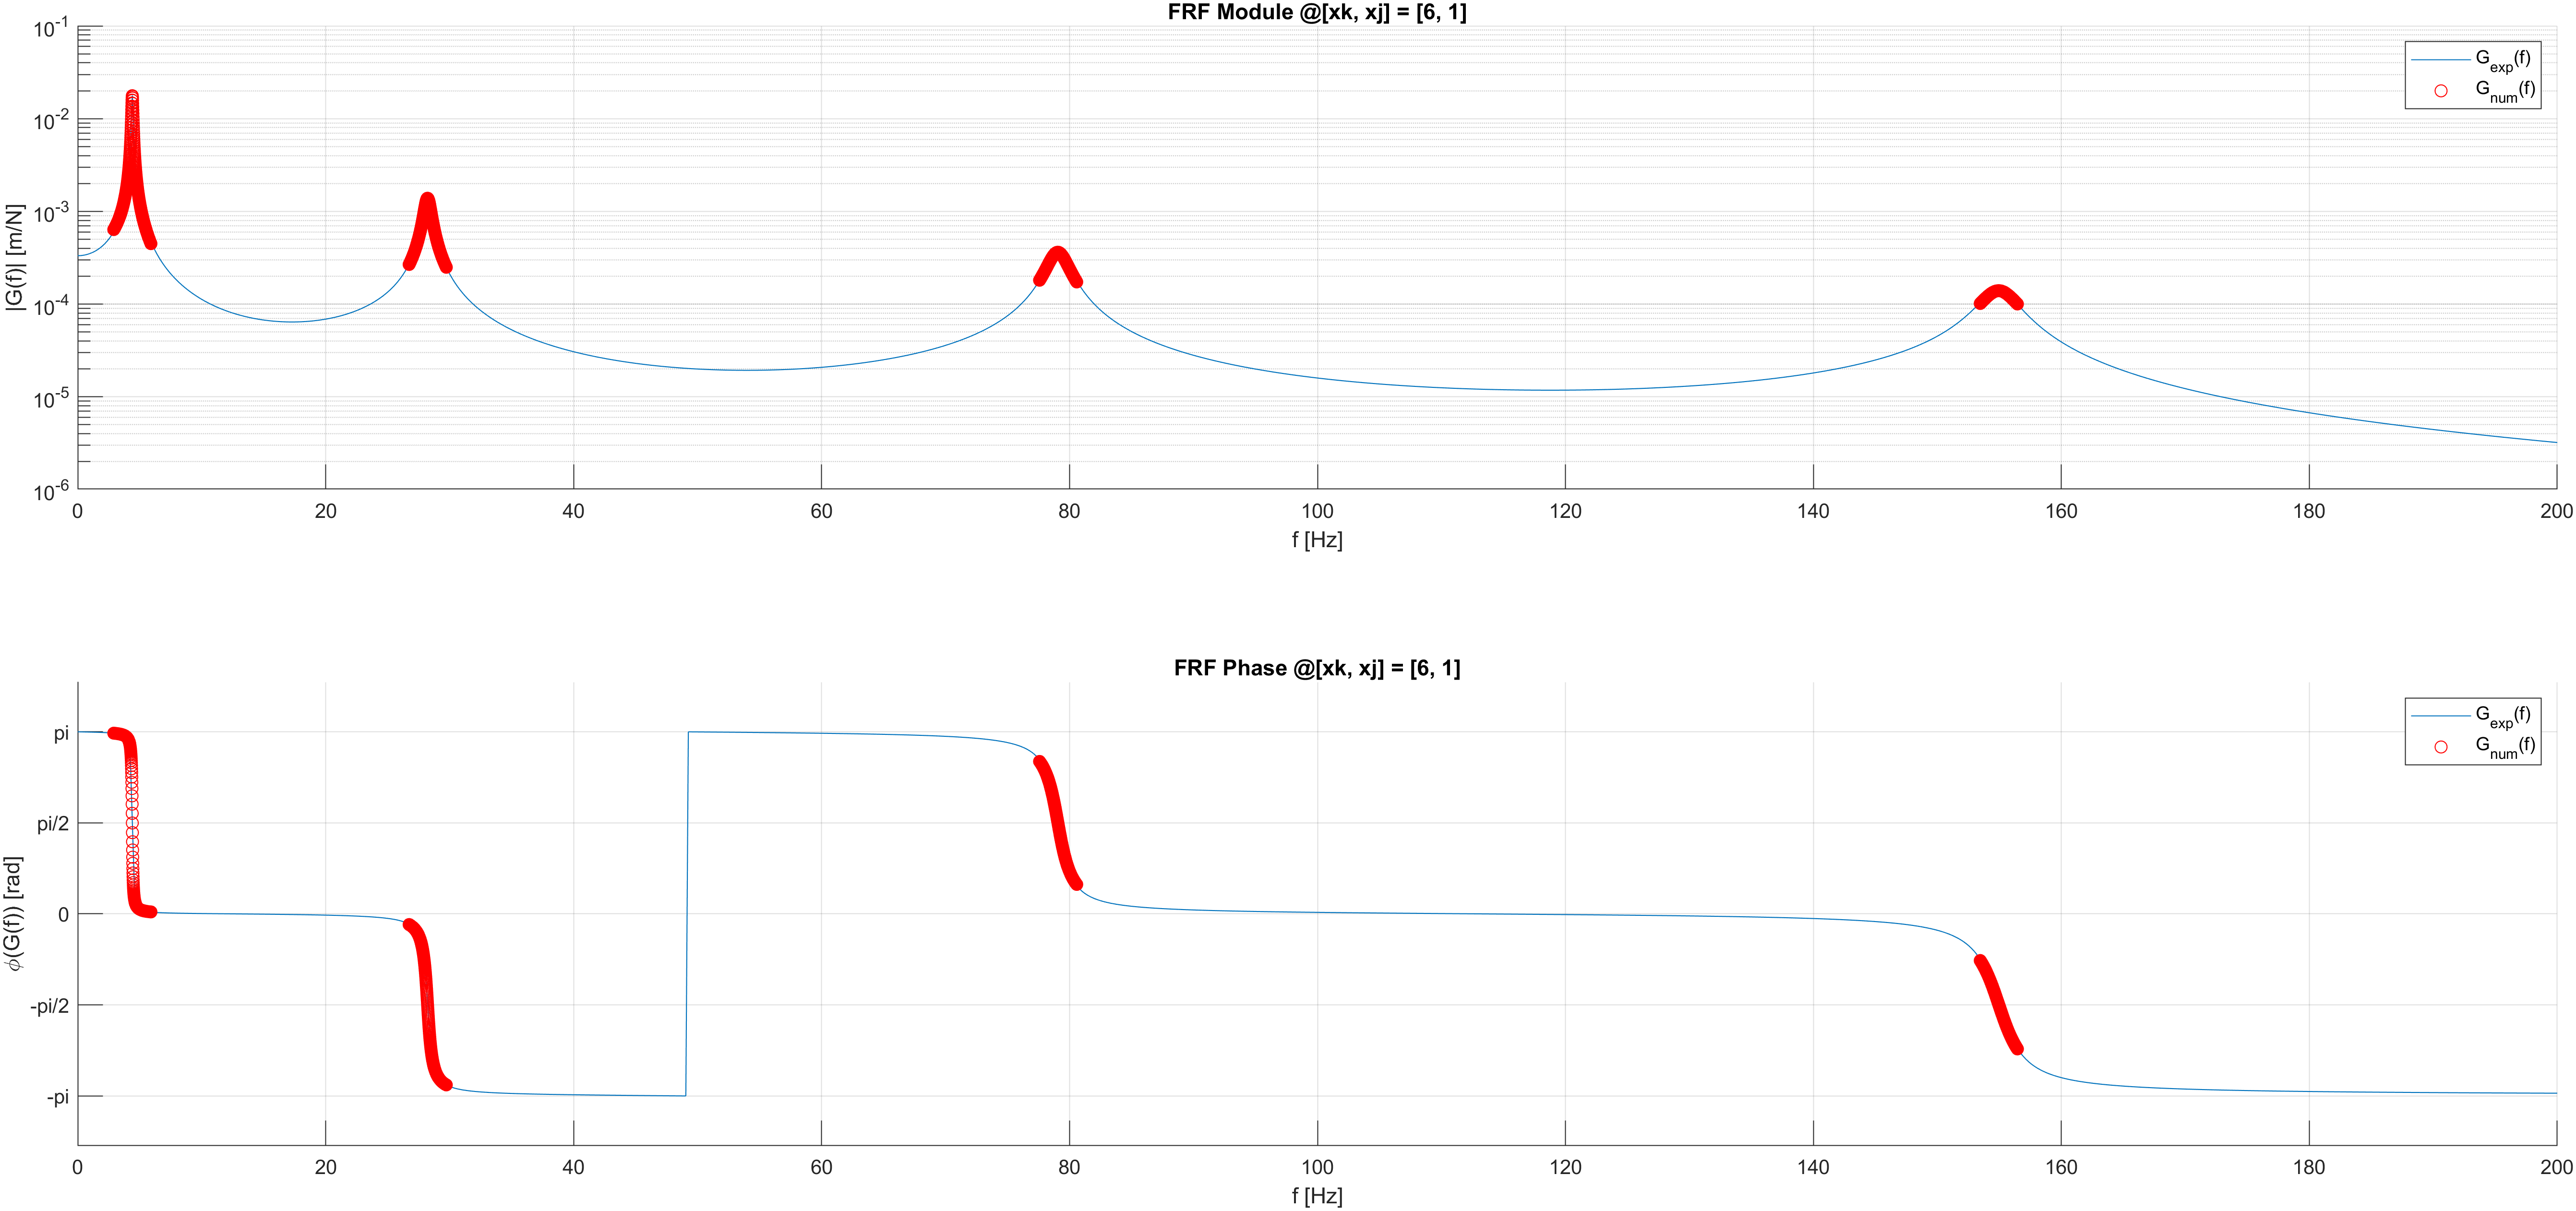
\includegraphics[width=\textwidth]{img/MATLAB/Part_A/Comparison_FRF_couple_1_6.png}
    \caption{FRF identification for $x_k = 1.0m$ and $y_j = 0.6m$}
    \label{fig:FRF_identification}
\end{figure}

\begin{center}
    \huge{Plot to be replaced with the 4 zooms over the 4 peaks.}
\end{center}

\begin{figure}[H]
    \begin{minipage}[b]{0.45\textwidth}
        \centering
        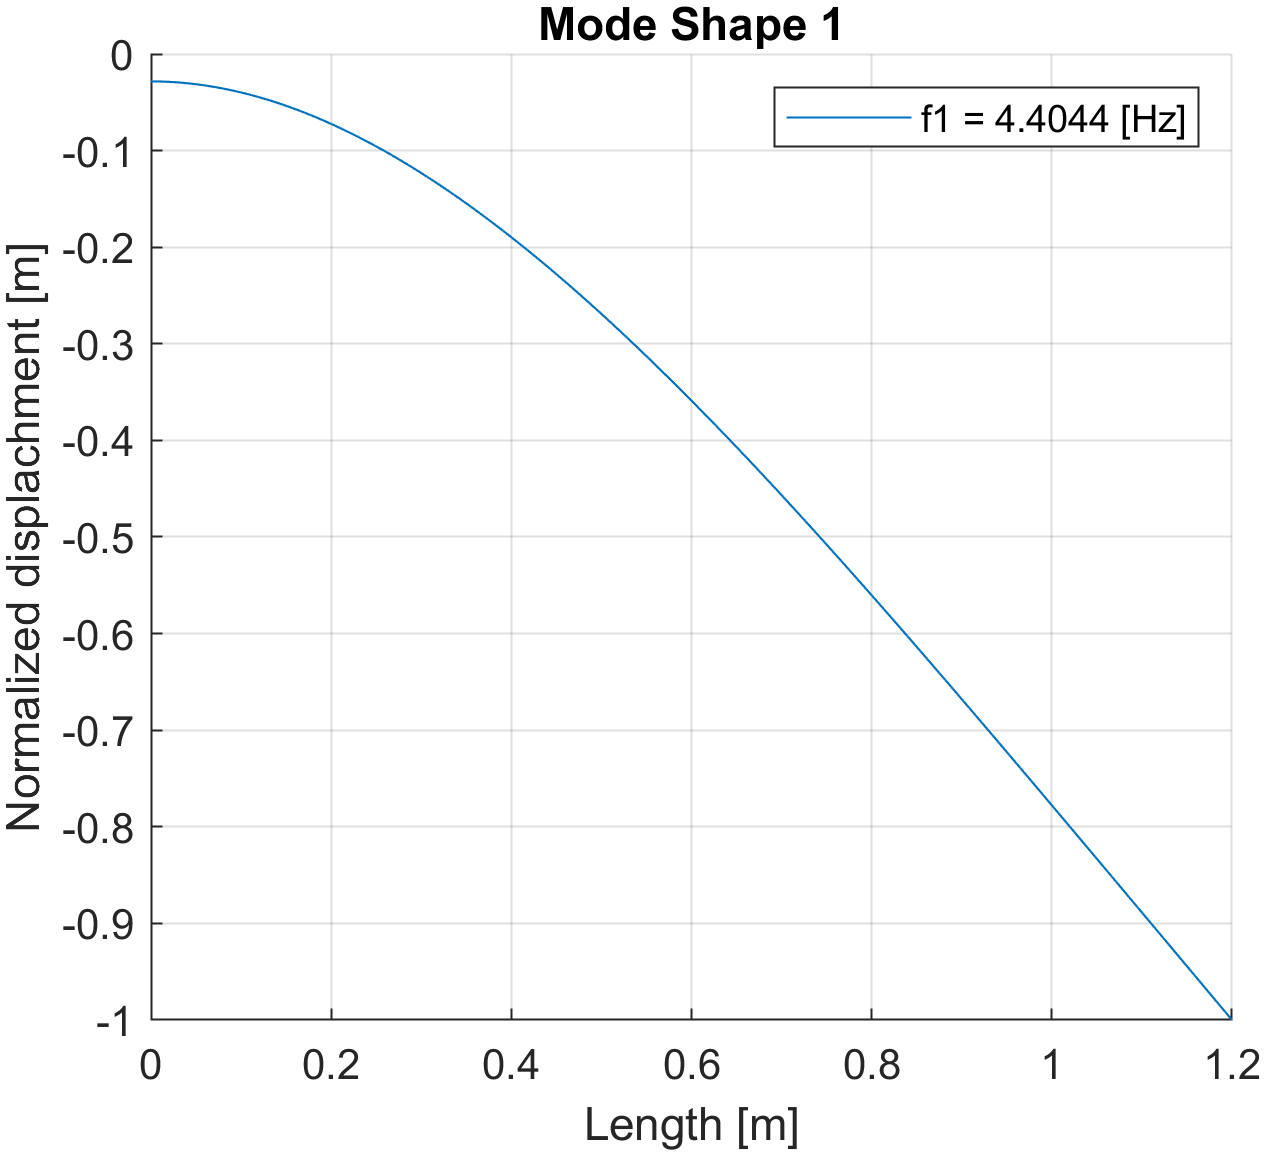
\includegraphics[width=\textwidth]{img/MATLAB/Part_A/Mode_shapes/mode_shape_01.png}
    \end{minipage}
    \hfill
    \begin{minipage}[b]{0.45\textwidth}
        \centering
        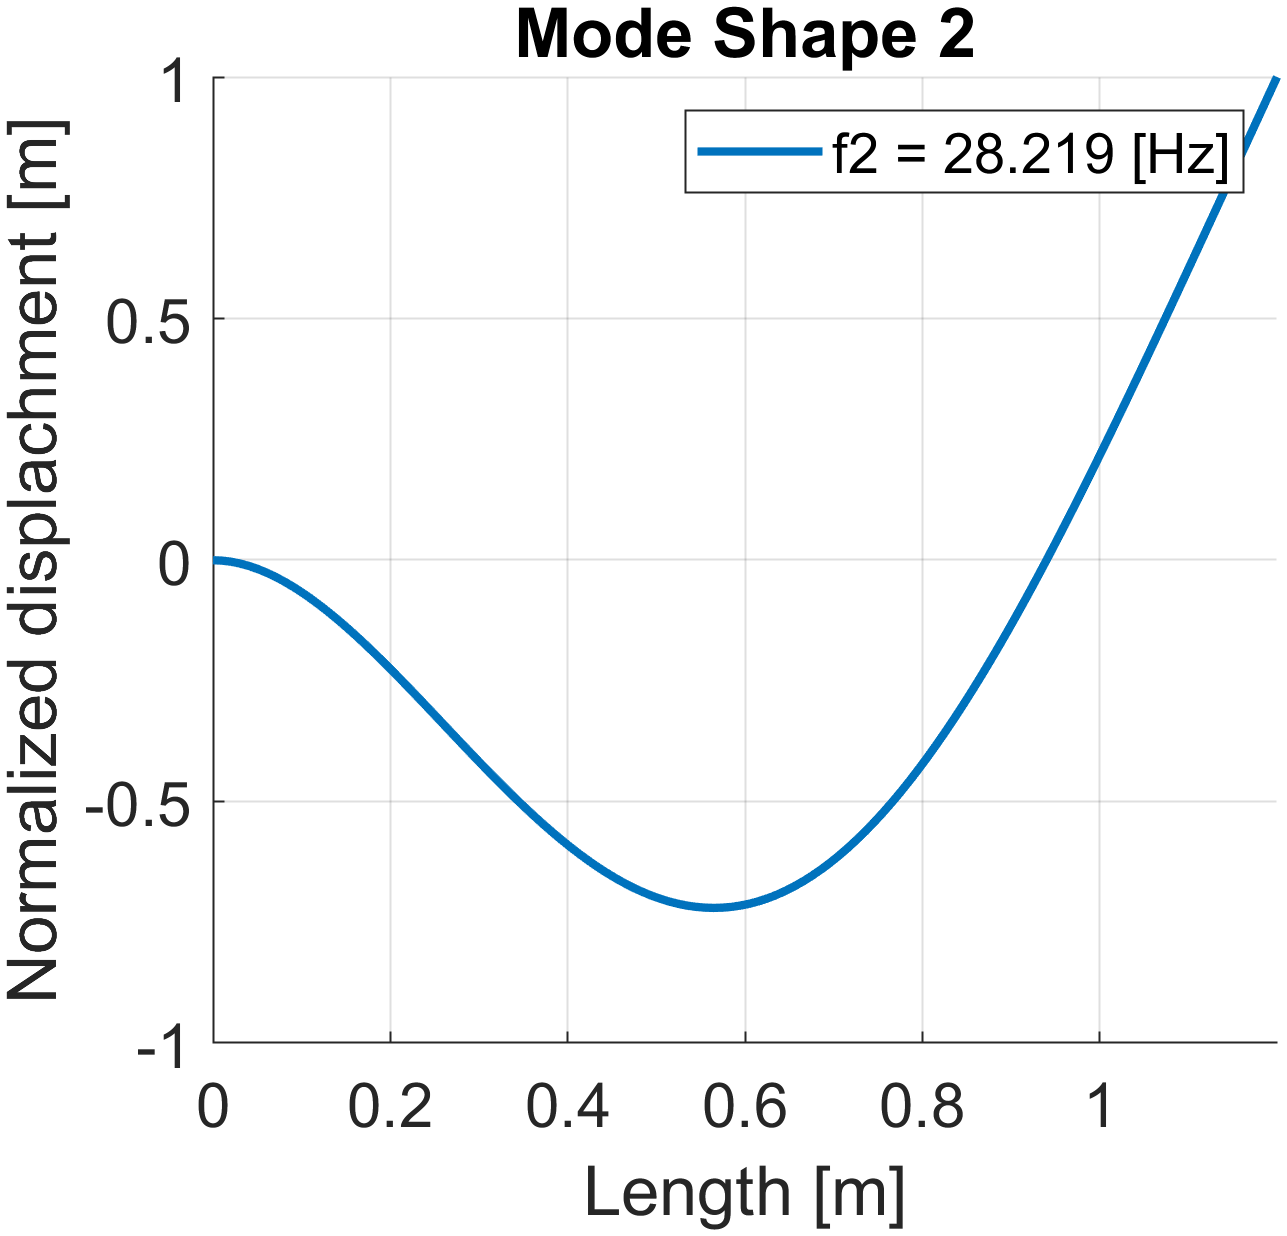
\includegraphics[width=\textwidth]{img/MATLAB/Part_A/Mode_shapes/mode_shape_02.png}
    \end{minipage}
    \begin{minipage}[b]{0.45\textwidth}
        \centering
        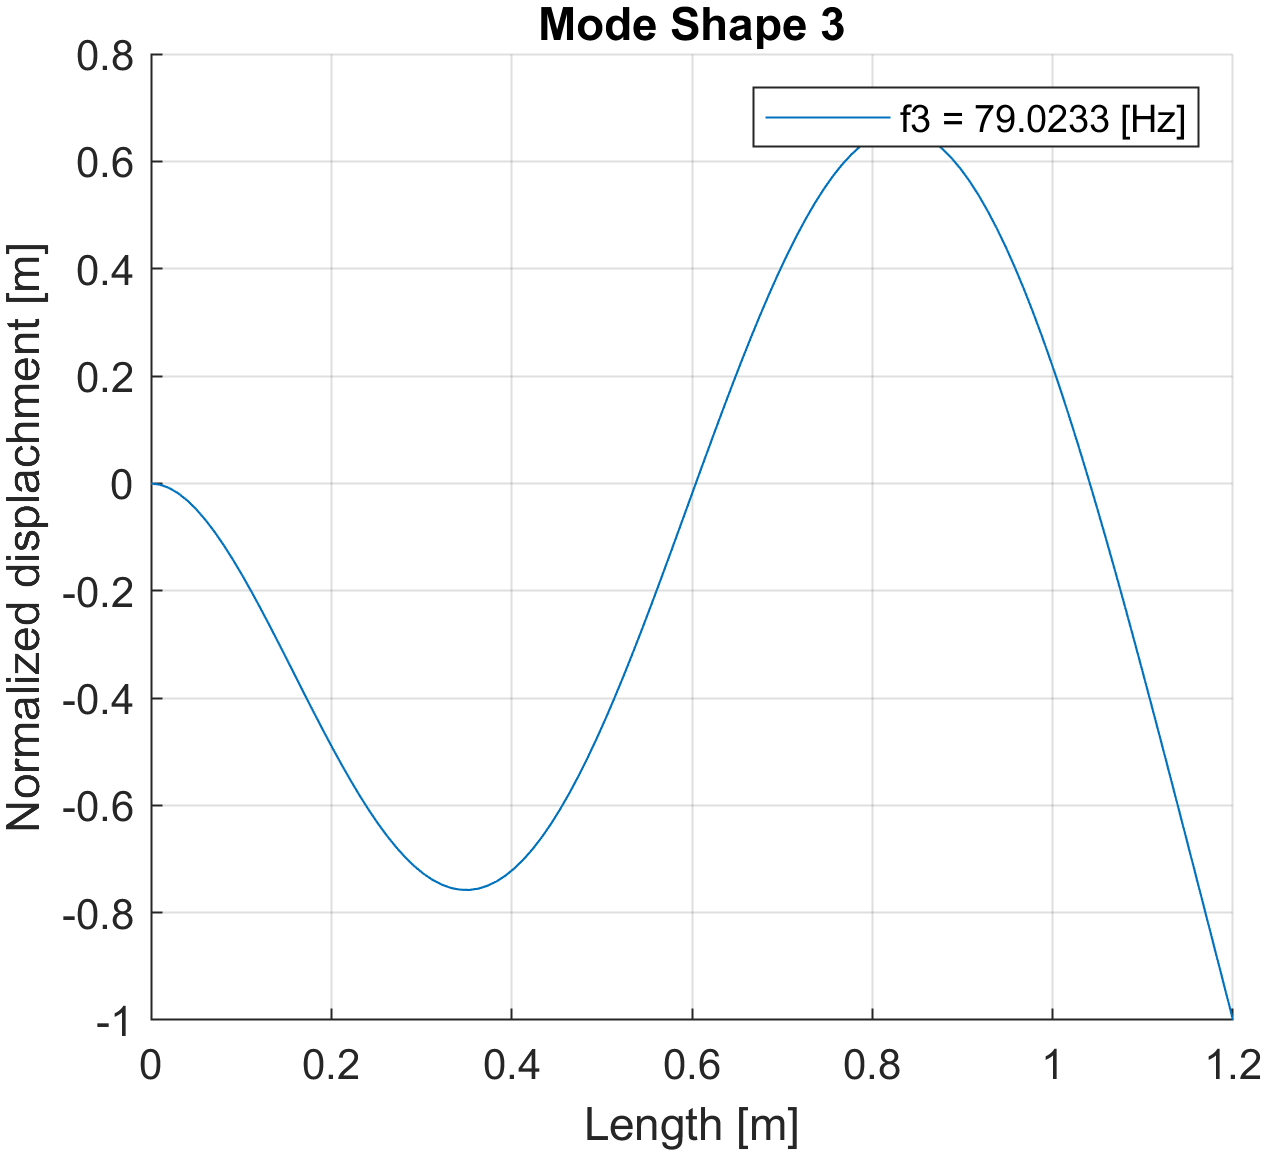
\includegraphics[width=\textwidth]{img/MATLAB/Part_A/Mode_shapes/mode_shape_03.png}
    \end{minipage}
    \hfill
    \begin{minipage}[b]{0.45\textwidth}
        \centering
        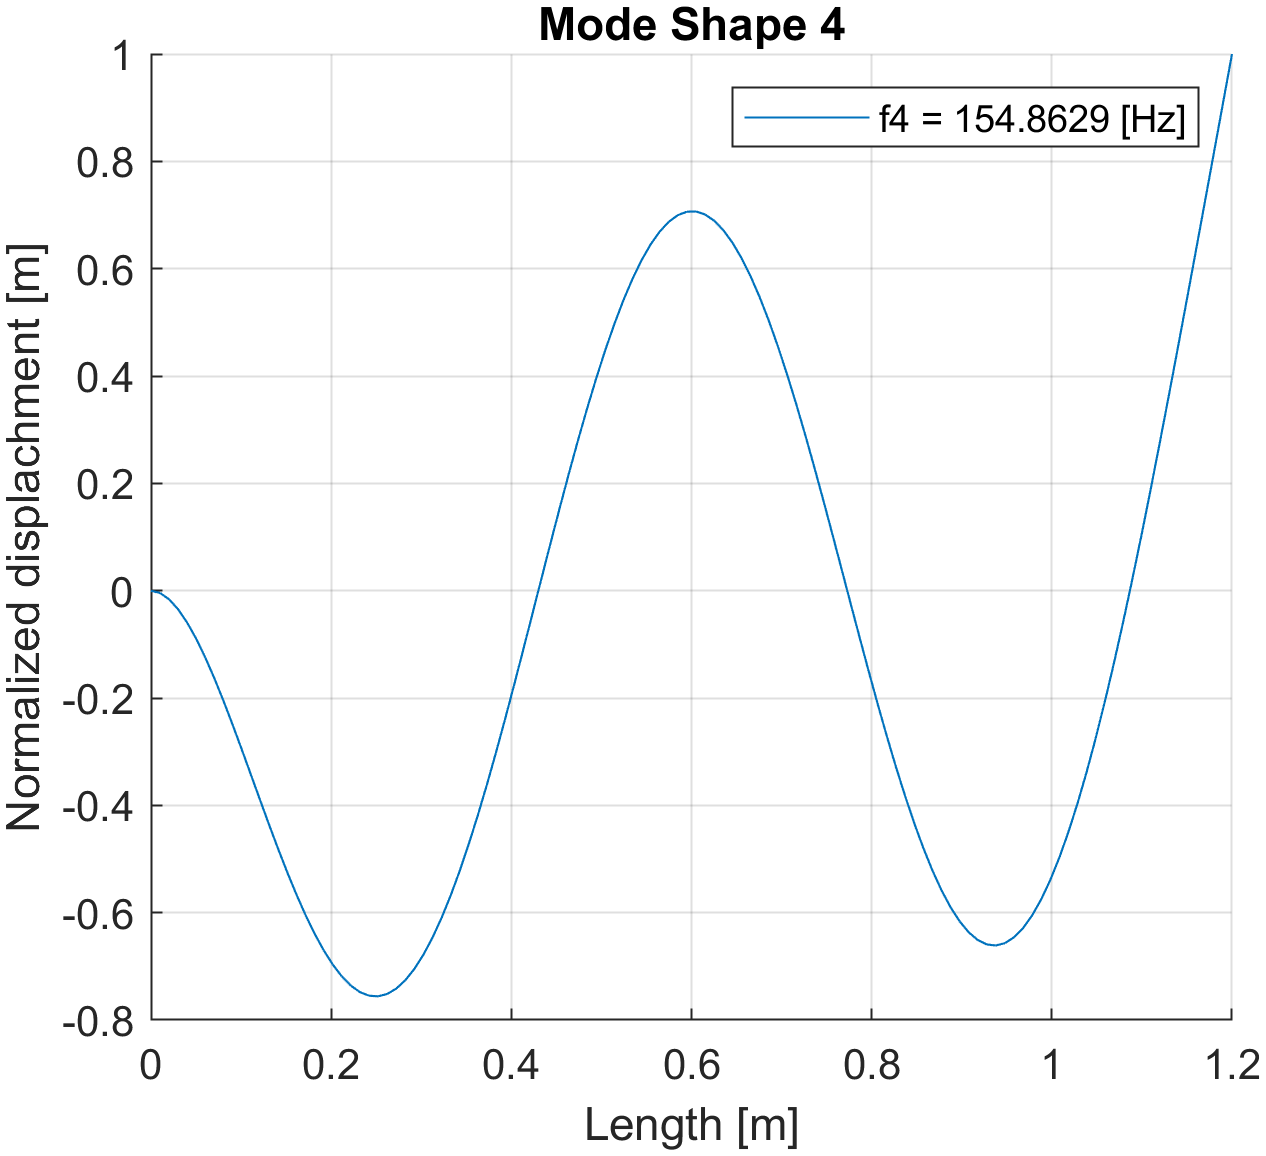
\includegraphics[width=\textwidth]{img/MATLAB/Part_A/Mode_shapes/mode_shape_04.png}
    \end{minipage}
    \caption{Zoom over the peaks of the FRF identification for $x_k = 1.0m$ and $y_j = 0.6m$}
    \label{fig:FRF_identification_zoom}
\end{figure}
